% PLIV candidate 1 -- Signal-weighted ATE identity (Theorem 1 / eqs. (2), (4))
\documentclass[border=4pt]{standalone}
\usepackage{amsmath,amssymb,bm,mathtools}
\usepackage{tikz}
\usetikzlibrary{positioning,calc,decorations.pathreplacing,arrows.meta,fit,backgrounds}
\usepackage{xcolor}
\definecolor{blue}{HTML}{1F618D}\definecolor{red}{HTML}{B03A2E}\definecolor{gray}{HTML}{7F7F7F}
\color[HTML]{111111}
\begin{document}
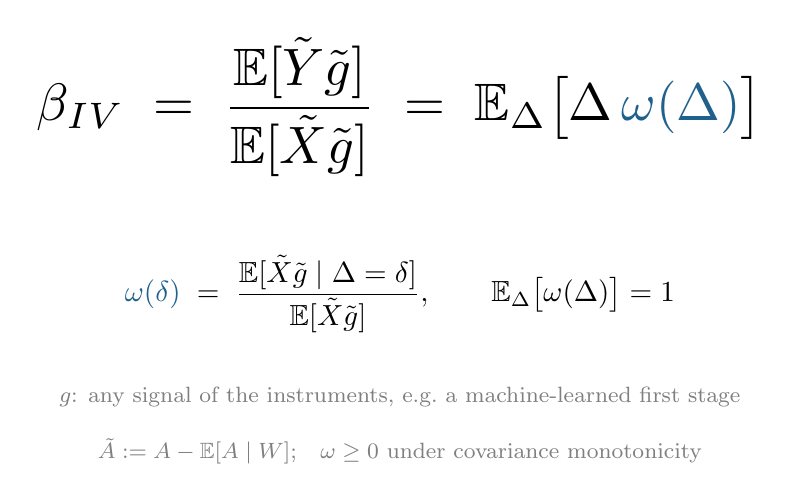
\begin{tikzpicture}
  % LINE 1 (dominant): eq. (4) ratio = eq. (2) / Theorem 1(i) representation
  \node (main) {\scalebox{1.9}{$\displaystyle
    \beta_{IV} \;=\; \frac{\mathbb{E}[\tilde Y \tilde g]}{\mathbb{E}[\tilde X \tilde g]}
    \;=\; \mathbb{E}_{\Delta}\big[\Delta\,{\color{blue}\omega(\Delta)}\big]$}};
  % LINE 2 (secondary): weight function, eq. (2); integrates to one, Theorem 1(ii)
  \node[below=7.5mm of main] (w) {\scalebox{1.05}{$\displaystyle
    {\color{blue}\omega(\delta)} \;=\; \frac{\mathbb{E}[\tilde X \tilde g \mid \Delta=\delta]}{\mathbb{E}[\tilde X \tilde g]},
    \qquad \mathbb{E}_{\Delta}\big[\omega(\Delta)\big]=1$}};
  % LINE 3 (grey): Theorem 1 holds for any measurable signal g
  \node[below=4.5mm of w, gray] (c1) {\footnotesize $g$: any signal of the instruments, e.g.\ a machine-learned first stage};
  % LINE 4 (grey): Robinson partialling (p.5) and Theorem 1(iii) under CCM
  \node[below=1.5mm of c1, gray] (c2) {\footnotesize $\tilde A := A-\mathbb{E}[A\mid W]$;\quad $\omega\ge 0$ under covariance monotonicity};
\end{tikzpicture}
\end{document}
